\documentclass{article}


% if you need to pass options to natbib, use, e.g.:
%     \PassOptionsToPackage{numbers, compress}{natbib}
% before loading neurips_2022


% ready for submission
% \usepackage{neurips_2022}


% to compile a preprint version, e.g., for submission to arXiv, add add the
% [preprint] option:
%     \usepackage[preprint]{neurips_2022}


% to compile a camera-ready version, add the [final] option, e.g.:
\usepackage[final]{neurips_2022}


% to avoid loading the natbib package, add option nonatbib:
% \usepackage[nonatbib]{neurips_2022}

\usepackage{array}
\usepackage{multirow}
\usepackage{floatrow}
\usepackage{graphicx}
\usepackage[utf8]{inputenc} % allow utf-8 input
\usepackage[T1]{fontenc}    % use 8-bit T1 fonts
\usepackage{hyperref}       % hyperlinks
\usepackage{url}            % simple URL typesetting
\usepackage{booktabs}       % professional-quality tables
\usepackage{amsfonts}       % blackboard math symbols
\usepackage{nicefrac}       % compact symbols for 1/2, etc.
\usepackage{microtype}      % microtypography
\usepackage{xcolor}         % colors


\title{Comparing Data-Guided Techniques for Enhancing Negation Sensitivity in MLM-Based Laguage-Models
}


% The \author macro works with any number of authors. There are two commands
% used to separate the names and addresses of multiple authors: \And and \AND.
%
% Using \And between authors leaves it to LaTeX to determine where to break the
% lines. Using \AND forces a line break at that point. So, if LaTeX puts 3 of 4
% authors names on the first line, and the last on the second line, try using
% \AND instead of \And before the third author name.


\author{%
  Philipp Koch
  % \thanks{Use footnote for providing further information
    % about author (webpage, alternative address)---\emph{not} for acknowledging
    % funding agencies.}
    \\
  Institute for Statistics\\
  Ludwig-Maximilians University\\
  Munich\\
  \texttt{P.Koch@campus.lmu.de} \\
  % examples of more authors
  % \And
  % Coauthor \\
  % Affiliation \\
  % Address \\
  % \texttt{email} \\
  % \AND
  % Coauthor \\
  % Affiliation \\
  % Address \\
  % \texttt{email} \\
  % \And
  % Coauthor \\
  % Affiliation \\
  % Address \\
  % \texttt{email} \\
  % \And
  % Coauthor \\
  % Affiliation \\
  % Address \\
  % \texttt{email} \\
}


\begin{document}


\maketitle


\begin{abstract}
Despite the recent success with LLMs in NLP, unsolved challenges in the field of NLU remain. The problem of misunderstanding the concept of negation in natural languages has been investigated in previous years and remains unsolved. Different solutions to alleviate the problem have been introduced recently. This work examines different novel approaches using data-based strategies while keeping as much of the initial - promising - MLM objective as possible. We generate artificial data using WordNet to construct a setup of two sentences in which things from the real world are described using a standard description and a description using negation and antonyms for an adversarial sample. Additionally, we also create a negation-overrepresenting dataset by filtering RoBERTa's pre-training data. We conduct four experiments using this data and different masking strategies. The results indicate that using our training data with unsupervised MLM leads to slight overall improvements. We also observe stark improvements (51\% to 62\%) in accuracy but also strong fluctuating behavior. Our model also improves accuracy on WNLI (13 \% to 41 \%), although it drops on many other GLUE tasks.
\end{abstract}


\section{Introduction}
\label{section:introduction}

In recent years, large language models  (LLMs) have proven to be a successful approach to solving many NLP-related problems. Especially the application of unsupervised learning on large amounts of data elevated the performance of LLMs (\cite{devlin-etal-2019-bert}, \cite{liu2019roberta}, \cite{brown2020language}). Specifically, the masked-language-model family has become a popular approach in natural language understanding (NLU) related tasks. Despite the unbroken success stories in many applications, some open problems remain regarding NLU. A particular issue in understanding is the concept of negation in natural languages, which may cause problems when it occurs in real-world applications. The problem has been the focus of research for quite some time (\cite{ettinger-2020-bert}, \cite{kassner-schutze-2020-negated}, \cite{hossain-etal-2020-analysis}, \cite{hossain-etal-2022-analysis}, but it has not been sufficiently solved to this day. Different approaches exist where the problem can be alleviated using different objectives (\cite{hosseini-etal-2021-understanding}, \cite{TruongImprovingNegation2022}). In this work, we investigate possible solutions approaching the problem mainly from the data side and investigate a supervised and unsupervised masking strategy to keep as much from the original - on many NLP-related tasks well-performing - MLM objective as possible.


\section{Masked-Language-Modeling}
\label{section::MLM}
Masked language modeling is a pre-training objective in NLP where a model is trained to predict a randomly masked word in a sentence based on the surrounding context. This technique was introduced by \cite{devlin-etal-2019-bert} based on \cite{taylor-cloze}. The aim is to train the model to learn contextual representations of words that can be fine-tuned for downstream NLP tasks.
The loss function used in masked language modeling is typically cross-entropy loss. The model generates a probability distribution over the vocabulary for each masked word and is optimized upon this prediction and the original token. 

\textbf{BERT} Bidirectional Encoder Representation Transformer (BERT) \citep{devlin-etal-2019-bert} is an encoder-only transformer model. The BERT model is trained on a large corpus of text data to learn contextual representations of words. This allows it to understand the meaning of a word in the context of the sentence it appears in. The model is bidirectional, meaning it can consider both the preceding and following words when generating a representation for a given word. BERT is trained using the MLM objective and next-sentence prediction. % 

\textbf{RoBERTa} In contrast to BERT, RoBERTa \citep{liu2019roberta} uses a different pre-training technique. The MLM objective and the share of masked words stay the same, but the training data is copied ten times, and the masks are applied randomly during training to allow the model to learn from different masking angles on the same sentence. Furthermore, the next-sentence prediction is dropped.

Both models achieved strong results and achieved state-of-the-art on various tasks at the time of their introduction.

\section{Understanding of Negation in Transformers}
\label{section::understanding}
The understanding capabilities of transformers have been extensively researched after the introduction of the BERT model. 
\cite{ettinger-2020-bert} conducted psycholinguistic experiments with it, including a task that examines the model's understanding of negation in natural language.
The task consists of a fill-in-blank task in which the model is expected to predict a token in a negated context. The sentences included unnatural and constructed samples but also natural-sounding sentences. An example for the (unnatural) task is the sentence: \textit{A robin is not a \texttt{MASK}}, where BERT-Large predicted: \textit{robin, bird, penguin, man, fly}. However, for sentences with negation, it was expected to predict anything but \textit{robin} or \textit{bird}.

Although this task seems trivial for a human, BERT had severe problems solving it (BERT-Base: 38.9\%, BERT-Large: 44.4\% accuracy).

A similar approach to examine BERT's capabilities concerning negation was conducted by \cite{kassner-schutze-2020-negated}. The focus of this work is on factual knowledge of LLMs. Akin to \cite{ettinger-2020-bert}, masked sentences were presented to the model for which the masked token was to be predicted. It was examined whether the model is capable of producing facts correctly. It was found that BERT (BERT-Base and BERT-Large) had a high overlap for correct and false answers when negation was added, which aligns with the findings of \cite{ettinger-2020-bert} of poor understanding of the concept of negation in BERT-models. However, it was also found that BERT can be improved in understanding negation when the model is fine-tuned in a supervised manner.

Further research was conducted regarding NLU corpora \citep{hossain-etal-2022-analysis}. It was found that negation does not appear in NLU corpora as commonly as in general-purpose English. Furthermore, negations are often unimportant to solving a task and do not even appear in some corpora. Models trained on these corpora yielded poorer results when they had to deal with tasks involving negation compared to tasks without negation.
Additionally, natural language inference benchmarks were also examined regarding the importance of negation \citep{hossain-etal-2020-analysis}, where it was found that negation is often underrepresented and can also be ignored in some benchmarks to obtain correct results.
A broader overview of the capabilities of LLMs was conducted by  \cite{lialin-etal-2022-life}. This work includes the broader BERT family and decoder- and encoder-decoder-based models. The models were evaluated on a wide range of linguistic tasks using the oLMpics dataset \citep{talmor-etal-2020-olmpics}, which also includes the task of antonym negation. It was found that RoBERTa obtained the highest value for the antonym negation task (RoBERTa-Large: 74.4\%).

\section{Related Work}
\label{section::rel_work}

Different approaches have already been introduced to alleviate the problem described in the previous section.

\cite{hosseini-etal-2021-understanding} introduced an approach to training BERT on the meaning of negation by supervision. In this procedure, sentences are negated using a negation module, e.g., "A is a B." becomes "A is not a B.". Knowing that the word \textit{B} is not desired at this position when also the first sentence is around, the model is trained to predict anything but \textit{B}, using unlikelihood loss \citep{welleck2019neural}:

$$ \mathcal L_{UL}(x_u) = - log(1 - p(x_B | x_{1:B-1})) $$

To further keep behavior from the original model, a distillation loss is used on unmodified samples, e.g., "A is a B." $\rightarrow$ "A is a B.":

$$ \mathcal L_{KL}(x_l) = D_{KL}(p_{LM}|| p) $$

In which $p$ is the distribution of tokens from the original model, while $p_LM$ is the distribution of the negation-aware model.
The fine-tuned model showed improved results on negation-sensitive tasks than the original BERT.

Another approach to improving BERT focused on negation understanding was introduced by \cite{TruongImprovingNegation2022}. This work presented two pre-training techniques; both improved the model's performance on data from the medical domain. Negation in the medical domain often plays a crucial role in understanding a problem.
For the first technique, the dataset is filtered, and only sentences with at least one negation are kept on which the model is subsequently trained using the model's original pre-training objective.
The other technique enhances the masked-language-modeling objective by adding a new \texttt{[CUE]} token, which is only used to mask negation cues. Based on this novel masking strategy, the model is expected to learn a more in-depth relation of negation in natural language. The following sentence exemplifies this approach. The sentence \textit{No serious complications such as hypertension, diabetes.} becomes \textit{\texttt{[CUE]} serious complications such as \texttt{[MASK]}, diabetes.} Both approaches show improvement over the original BERT on some tasks.


\section{Novel Techniques to Improve Understanding of Negation}
\label{section::questions}

This work aims to answer two questions regarding potential modifications in pre-training data to improve the model's capabilities with respect to the concept of negation.

\textbf{Question 1: Does it suffice to train an LLM on data in which negation is overrepresented?} Previous work (\cite{hossain-etal-2022-analysis}, \cite{TruongImprovingNegation2022}) indicates that this approach might help improve the model's overall negation understanding, and it was found that negation is underrepresented in many corpora \citep{hossain-etal-2022-analysis}. To our knowledge, this approach had not been tested on the general pre-training data. Using this negation-aware data in general pre-training might improve the model.

\textbf{Question 2: Can the model learn the concept of negation when specific (negation-aware) data is injected into the training data?}\label{question2}
The work of \cite{kassner-schutze-2020-negated} and \cite{hosseini-etal-2021-understanding} indicates a setup in which negation is passively explained through adversarial examples improves the model. Can this be potentially also used for general pre-training?

Due to the strong generalizability of the MLM objective, we deliberately try to be as close as possible to the initial MLM training and not modify the loss. The aim is to investigate if the current MLM pre-training objective can be enhanced using a different data-strategy.


\section{Experiments}
\label{section::experiments}

Three experiments will be conducted to answer the questions from the previous section. We train the model for three epochs and use the AdamW optimizer \citep{loshchilov2019decoupled} for optimization in all experiments. We evaluate the model after ten thousand steps each and observe the behavior during training. Further hyperparameters are reported in the appendix.

\textbf{Experiment 1:}
Training of BERT-Small on negation-aware (filtered) pre-training data of RoBERTa using the MLM objective (the selection of RoBERTa is intentional here since the highest score on the oLMpics antonym-negation task was achieved by this model). This experiment is similar to \cite{TruongImprovingNegation2022}. However, we do not only train on domain-specific data but on the filtered pre-training data. Furthermore, we choose all sentences with at least one negation and their adjacent context of 2 neighboring sentences on each side.

\textbf{Experiment 2}
We train BERT-Small on adversarial data similar to \cite{hosseini-etal-2021-understanding} and \cite{kassner-schutze-2020-negated}. Furthermore, we use instances from the filtered training data to avoid overfitting the artificial, adversarial training data. We apply supervised masking on the adversarial training data in which either the antonym or the word itself is masked. The model predicts the token based on the initial description and the negated description with the antonym. The setup is similar to \cite{hosseini-etal-2021-understanding} but uses cross-entropy loss for optimizing the predictions to be closer to the original objective (because we have prior knowledge about the antonyms). At the same time, we keep random masking for filtered data.

\textbf{Experiment 3}
Instead of supervised masking on the adversarial data, we now mix filtered and adversarial data and use the MLM objective on the combined dataset in another attempt to test if masking words randomly is sufficient to improve the model's performance, approaching the problem entirely from the data.

The selection of BERT-Small is due to computational resources. We freeze the first three encoder layers of BERT-Small only to tune the upper layers. It was found that semantic knowledge is stored in the upper layers \citep{jawahar-etal-2019-bert}, which we want to modify. For the implementation of the experiments, we use the transformers library \citep{wolf-etal-2020-transformers} for this work.

\section{Data}
\label{section::data}
In this section, we will describe the data on which the experiments will be conducted. We use three datasets, of which two are solely for training and of which one is only for evaluation. 

\subsection{RoBERTa's Pre-Training Data}
% PROOFREAD
Due to the results in Lialin et al., that showed high accuracy of RoBERTa in antonym negation, we take the pre-training data of RoBERTa. RoBERTa was trained on five different datasets of which only four where available at the time of this work. The datasets used in this work are: 

10\% of available datasets (listed in the appendix) of the RoBERTa-Pre-Training dataset is searched for negations using spaCy's linguistic parser \citep{Honnibal-Spacy-2017}. A short descriptive analysis of the results we found is provided in \ref{tab:data_stats} (appendix).

For our purpose, we filter the dataset. All sentences that include a negation are collected. Since the context is assumed to be also required for the understanding of the negated phrase, we also add the previous two and the subsequent two sentences to the dataset. Using this technique, we can increase the share of sentences with negation to over 20\%. An example of an instance from the filtered data can be seen in the appendix in Table \ref{tab:filtered_data_example}. We will also refer to this data as \textit{filtered data}.

\subsection{Synthetic Data based on WordNet}
Another approach is training the model using an adversarial data-setup, in which a sentence is used as an adversarial reference to teach the model the usage of negation. \cite{hosseini-etal-2021-understanding} used unlikelihood loss for the adversarial reference sentence in which the word from the original sentence needs to be as far away from the antonym as possible in the latent space. \cite{kassner-schutze-2020-negated} use a knowledge base to construct artificial sentences on which later BERT is trained in a supervised manner.

Our approach is similar, although no additional loss function will be used, and the knowledge base we are using is WordNet (\cite{miller-1994-wordnet}, \cite{fellbaum-wordnet1998}, \cite{princeton-wordnet-online}). 
Both sentences describe something in the real world. The first sentence does this by simply stating the fact and the other sentence describes what the previous description is not by using negation and the antonym of the word in the initial sentence. Using this adversarial setup, we supply the model with an indirect description of how negation works in natural language. Table \ref{tab:wn_example} shows an example of these sentences.
Akin to the approach in \cite{kassner-schutze-2020-negated}, we build an artificial dataset by filling in templates using all available nouns, adjectives, and their respective antonyms from the WordNet database. Verbs have not been used due to the difficulty of inflection in template-based systems.
We used the NLTK \citep{bird2009natural} and checklist \citep{ribeiro-etal-2020-beyond} library to implement the dataset generator.
Our dataset contains 755200 sentences and can be used in a supervised and unsupervised setup. An example of an instance of the supervised and unsupervised setup can be found in table \ref{tab:wn_example}.
We will refer to this data as \textit{WordNet adversarial data}.

\begin{table}[!h]
    \centering
    \small
    \begin{tabular}{c|c}
            & Data\\ \hline
            Original                    & \texttt{This is a maximum. This isn't a minimum.} \\
            \multirow{2}{*}{Supervised} & \texttt{This is a maximum. This isn't a [MASK].} \\
                                        & \texttt{[REF-BEG] minimum [REF-END]} \\
            Unsupervised MLM            & \texttt{This [MASK] a maximum. This isn't a minimum.} \\ 
    \end{tabular}
    \caption{Example of an instance of WordNet adversarial data. (Special tokens in the supervised masking example are used to construct the labels during dataset instantiation.)}
    \label{tab:wn_example}
\end{table}

\subsection{oLMpics Dataset for Evaluation}
We use the oLMpics antonym negation task \citep{talmor-etal-2020-olmpics} to evaluate the model, similar to \cite{lialin-etal-2022-life}. This dataset consists of linguistic tasks in which the model has to predict a particular masked word. Since this prediction is a classification problem, accuracy is used as a metric.
An example of an instance of the antonym negation task is: \textit{It was \texttt{[MASK]} hot, it was really cold.}.


\section{Results}
\label{section::results}
The results of the trained BERT-Small model are reported in \ref{tab:results} and must be viewed in comparison to the baseline of 51 \% accuracy on the oLMpics antonym negation task of the original BERT-Small model. For experiments 1 to 3, we refer to the appendix for the evaluation graphs.

\begin{table}[!h]
    \centering
    \begin{tabular}{l|c|c|c|c}
        \hline
                    & Experiment 1      & Experiment 2          & Experiment 3 (avg.)   & Experiment 3+     \\ \hline
                    &                   &                       &                       &                   \\
        Final Value & 0.504             & 0.518                 & 0.520                 & 0.548             \\
        Best Value  & \textbf{0.530}    & \textbf{0.528}        & \textbf{0.557}        & \textbf{0.620}    \\ \hline
    \end{tabular}
    \caption{Results of the three experiments and the additional experiment 3+ based on experiment 3.}
    \label{tab:results}
\end{table}


\textbf{Experiment 1}
Using only the filtered data to train BERT-Small with MLM objective did not improve the model significantly. At the beginning of the training, we observed slight fluctuation in which the performance rose to 53\% accuracy at one evaluation step and dropped to the lowest point of 50.2\% accuracy. After the 60th step, however, we observed stable behavior below the baseline of 51\% accuracy. Eventually, the training converges to 50.04\% accuracy. 

\textbf{Experiment 2}
Training BERT-Small on WordNet adversarial data with supervised masking and on filtered data using unsupervised MLM also showed no improvement. The accuracy improved to 52.8\% and dropped at the lowest point to 50\% accuracy. Our final result was 51.8\% accuracy, improving over the baseline of 51\% by 0.8\% percentage points. The training data used here was considerably smaller than in experiment 1.

\begin{figure}[!htbp]
    \centering
    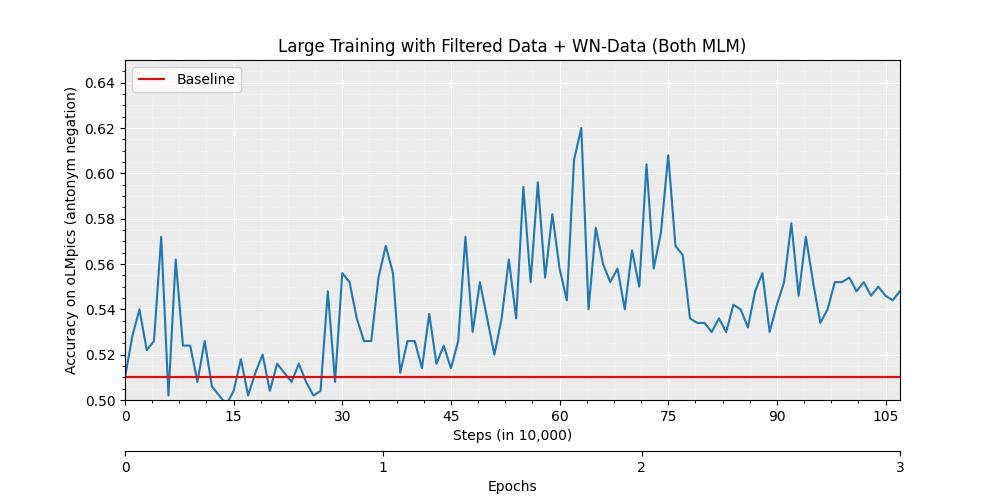
\includegraphics[width=\textwidth]{figures/Large_Training_with_Filtered_Data___WN_Data__Both_MLM_.jpg}
    \caption{Evaluations during training of experiment 3+. Despite some stark improvements, the fluctuations also cause severe drops.}
    \label{fig:exp3}
\end{figure}

\textbf{Experiment 3}
Training BERT entirely with an unsupervised MLM objective on both filtered and training data yielded a different behavior in contrast to the previous experiments. We trained the model three times using different seeds to validate this behavior.
During the first steps in the first epoch, we observed stark fluctuations in accuracy for all three runs. The best value on average we obtained during the three runs was 55.7\% accuracy, while the largest value in accuracy on an individual run was 57.2\%. Although the values considerably increased, the behavior was unstable during this period (Epoch 1 in \ref{fig:exp3}, appendix). In the latter two-thirds of the training, we observe a drop in accuracy while the fluctuations weaken and the procedure stabilizes. The average value of the three runs obtained at the end was 52\% accuracy, which is a slight improvement over the baseline (51\% accuracy). The training data used in this experiment included the same amount of instances as experiment 2.

\textbf{Experiment 3+}
Due to the improvement seen in Experiment 3, we tested another approach based on the pre-training strategy in RoBERTa. To further supply the model with even more data, we also copied the WordNet adversarial data ten times, so the sentences can be masked and thus learned from different angles as introduced by \cite{liu2019roberta}. Due to this procedure, the dataset size also increased substantially, limiting us to only train the model once.
This experiment yielded an overall better result than the previous experiments. The highest value we obtained was 62\% accuracy, while the lowest was 49.8\% accuracy. We found even more fluctuations during training that continued into the second epoch than in the previous experiments, as seen in \ref{fig:exp3}. The magnitude of the fluctuations were multiple percentage points. After the maximum value of 62\% accuracy was reached, the model dropped in the next step to 54\%. This unstable behavior stopped during the last epoch when the accuracy became more stable at a higher value than the baseline. Finally, the training finishes with an accuracy of 54.8\%, which is an improvement of 3.8 percentage points over the baseline.

Throughout all experiments, we could not observe a clear upwards trend in accuracy (but a downward trend for experiment 1). The first two experiments did not deviate by more than 0.8\% points from the baseline eventually. In comparison, the last two experiments partially caused an increase of multiple percentage points. However, both experiments showed stark unstable behavior at the beginning of the training, where the highest values were observed. Eventually, both approaches (exp. 3 and exp 3+) led to a slight improvement after training.

\section{Evaluation on GLUE}
\label{section::glue}

\begin{table}[!h]
    \centering
    \begin{tabular}{l|l|cc}
                                                        & Metric        & Original      & Ours   \\ \hline
        \multirow{2}{*}{Microsoft Research Paraphrase Corpus (MRPC)}     & Accuracy      & \textbf{0.79}          & 0.66   \\
                                                        & F1            & \textbf{0.86}          & 0.76   \\ \hline
        The Corpus of Linguistic Acceptability (COLA)   & Matthews Corr. Coeff.     & \textbf{0.36}          & 0.12 \\ \hline
        Winograd Natural Language Inference (WNLI)      & Accuracy      & 0.13          & \textbf{0.41} \\ \hline
        Question Natural Language Inference (QNLI)      & Accuracy      & \textbf{0.86}          & 0.57  \\ \hline
        \multirow{2}{*}{Quora Question Pairs (QQP)}     & Accuracy      & \textbf{0.90}          & 0.82 \\ 
                             & F1            & \textbf{0.86}          & 0.77 \\ \hline
        
        Recognizing Textual Entailment (RTE)            & Accuracy      & \textbf{0.65}          & 0.51 \\ \hline
        The Stanford Sentiment Treebank (SST)           & Accuracy      & \textbf{0.88}          & 0.79 \\ \hline
    \end{tabular}
    \caption{Results for the evaluation on selected GLUE tasks.}
    \label{tab:glue}
\end{table}

To verify whether the performance of the model is still kept after applying experiment 3+, we evaluate the final model on selected GLUE tasks \citep{wang-etal-2018-glue} \footnote{MRPC \citep{dolan2005automatically}, COLA \citep{warstadt2018neural}, WNLI \citep{levesque2012winograd}, QNLI \citep{rajpurkar-etal-2016-squad}, QQP \citep{iyer-qqp-2016}, RTE (\cite{dagan-rte-2006}, \cite{haim2006second}, \cite{giampiccolo-etal-2007-third}, \cite{bentivogli2009fifth}), SST \citep{socher-etal-2013-recursive}}. Keeping the model competitive failed for most tasks, where our model dropped compared to the original BERT-small model. However, for the Winograd NLI Challenge \citep{levesque2012winograd} we observe a stark improvement by more than threefold. The results are reported in table \ref{tab:glue} and the hyperparameters for fine-tuning are reported in \ref{tab:glue-ft} (appendix).

\section{Discussion and Limitations}

The validity of this work remains limited due to computational limitations that constrained the use of costly experiments and validations. Only experiment 3 was trained using three different seeds, where similar behavior between the training runs was observed. However, this was not possible for other experiments, which were too costly. Due to this limitation, it was also not feasible to explore the limits of the current state-of-the-art model (RoBERTa-Large), which might have behaved differently. Furthermore, the usage of large datasets was thus also not possible, and thus only 10\% of the pre-training data of RoBERTa was used for experiment 1.
Another limitation following this problem is the absence of strong augmentation models for WordNet adversarial data. While it was possible to generate data using nouns and adjectives by filling in templates, this did not work for verbs, for which inflection is necessary.

\section{Conclusion}

Although some improvements have been seen, the results remain still close to guessing. The final values of all experiments remain close to the initial baseline and at 50\% accuracy. Furthermore, the fluctuating behavior during training weakens the power of the more significant improvements during training, especially shown by the sharp drop after achieving 62\% accuracy down to 54\%.
Returning to the questions from section \ref{section::questions}, we can not conclude that training solely on data in which more negation appears alleviates the problem (\textbf{question 1}). However, for \textbf{question 2}, we can see a slight improvement when training a model on the adversarial data, although the overall performance on general benchmarks (selected GLUE-tasks) drops.
The slight improvement as soon as WordNet adversarial data is introduced aligns with the results of previous work (\cite{kassner-schutze-2020-negated}, \cite{hosseini-etal-2021-understanding}), which also shows improvement using this setting. Similar to \cite{TruongImprovingNegation2022}, our approach of using filtered data from original pre-training and artificial adversarial data might be helpful to warm up models before fine-tuning them on negation-intense tasks as in the medical domain. Further research in this direction is highly appreciated.
The proposed technique of training an MLM-based model on filtered and adversarial data significantly improved the model's capability in solving the Winograd NLI challenge. Our model achieves a more than threefold increase in accuracy on WNLI compared to the original BERT-Small, implying that the proposed technique might also be helpful in other tasks besides improving the model's negation understanding.
The computational constraint problem also limits this work's validity. Thus, we recommend replicating the experiments using current state-of-the-art models and augmentation for WordNet adversarial data to also use verbs in the dataset.

\bibliography{bibliography}
\bibliographystyle{dcu}


\appendix


\section{Appendix}

\subsection{Filtered Data}

\subsubsection{Available RoBERTa Pre-Training Datasets}
\begin{itemize}
    \item BookCorpus \citep{Zhu_2015_ICCV}
    \item English Wikipedia (Version 2022/03/01, \cite{wikidump}
    \item CC-News \citep{Hamborg2017}
    \item OpenWebText \citep{Gokaslan2019OpenWeb}
\end{itemize}

\subsubsection{Descriptive Analysis of Negation in RoBERTa Pre-Training-Data}
\begin{table}[!h]
    \centering
    \begin{tabular}{l|c}
        Dataset         & Sent. w Negation (in \%) \\ \hline
        Wikipedia       & 5 \\
        BookCorpus      & 17 \\
        CC-News         & 12 \\
        OpenWebText     & 16 \\
        Total           & 11 \\
    \end{tabular}
    \caption{Percentage of negations in datasets used in RoBERTa pre-training}
    \label{tab:data_stats}
\end{table}

The amount of sentences with negations aligns with the findings of \cite{hossain-etal-2022-analysis} as there is also a misrepresentation compared to general-purpose English in which negation occurs more often (22.6\%–29.9\%, \cite{hossain-etal-2022-analysis}).
\newpage

\subsubsection{Example}
\begin{table}[!h]
    \centering
    \begin{tabular}{l|l}
        Includes Negation ? & Sentence \\ \hline
         w/o negation   & emma rolled her eyes .  \\
         w/o negation   & `` i 'm very satisfied with both my choices , megan . \\
         w negation     & you do n't have to worry . '' \\
         w/o negation   & `` so who is the godfather again ? \\
         w negation    & he 's not part of the family . ''
    \end{tabular}
    \caption{Example of an instance of the filtered dataset from RoBERTa pre-training data.}
    \label{tab:filtered_data_example}
\end{table}

\subsection{Hyperparameters - Experiment 1}
\begin{table}[!h]
    \centering
    \begin{tabular}{r|l}
        Parameter & Value \\ \hline
        Model Identifier (transformers library) & \texttt{prajjwal1/bert-small} \\
        Optimizer & AdamW \\
        Learning Rate & 5e-5 \\
        Epochs & 3 \\
        Batch Size & 16 \\
        Blocksize & 128 \\
        Data Collator for Training & \texttt{DataCollatorForLanguageModeling} (transformer library) \\
        Test Ds. Proportion & 5 \\
        Steps (Evaluation) & 10000 \\
        seed & 42 \\
        Layers Frozen & 0, 1, 2 \\
         \multirow{16}{*}{Frozen Layers} &     bert.encoder.layer.\{0,1,2,\}.attention.self.query.weight \\
                      &      bert.encoder.layer.\{0,1,2,\}.attention.self.query.bias \\
                      &      bert.encoder.layer.\{0,1,2,\}.attention.self.key.weight \\
                      &      bert.encoder.layer.\{0,1,2,\}.attention.self.key.bias \\
                      &      bert.encoder.layer.\{0,1,2,\}.attention.self.value.weight \\
                      &      bert.encoder.layer.\{0,1,2,\}.attention.self.value.bias \\
                      &      bert.encoder.layer.\{0,1,2,\}.attention.output.dense.weight \\
                      &      bert.encoder.layer.\{0,1,2,\}.attention.output.dense.bias \\
                      &      bert.encoder.layer.\{0,1,2,\}.attention.output.LayerNorm.weight \\
                      &      bert.encoder.layer.\{0,1,2,\}.attention.output.LayerNorm.bias \\
                      &      bert.encoder.layer.\{0,1,2,\}.intermediate.dense.weight \\
                      &      bert.encoder.layer.\{0,1,2,\}.intermediate.dense.bias \\
                      &      bert.encoder.layer.\{0,1,2,\}.output.dense.weight \\
                      &      bert.encoder.layer.\{0,1,2,\}.output.dense.bias \\
                      &      bert.encoder.layer.\{0,1,2,\}.output.LayerNorm.weight \\
                      &      bert.encoder.layer.\{0,1,2,\}.output.LayerNorm.bias \\
    \end{tabular}
    \caption{Hyperparameters used in Experiment 1. All values that are not reported, are default values from the transformer library.}
    \label{tab:hyp_exp1}
\end{table}
\newpage

\subsection{Evaluation Graph - Experiment 1}
\begin{figure}[!h]
    \centering
    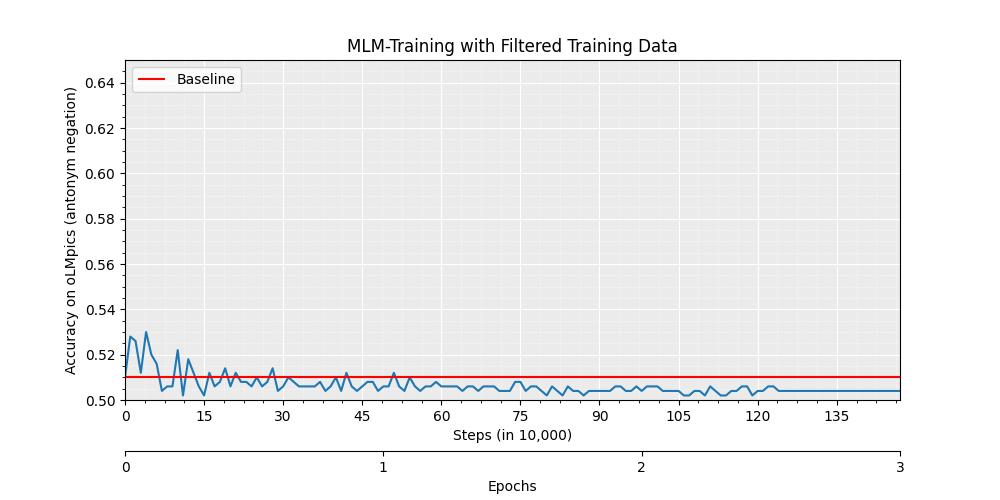
\includegraphics[width=\textwidth]{figures/MLM_Training_with_Filtered_Training_Data.jpg}
    \caption{Experiment 1: Training BERT-Small on the filtered dataset.}
    \label{fig:graph_exp1}
\end{figure}

\subsection{Hyperparameters - Experiment 2}
\begin{table}[!h]
    \centering
    \begin{tabular}{r|l}
        Parameter & Value \\ \hline
        Model Identifier (transformers library) & \texttt{prajjwal1/bert-small} \\
        Optimizer & AdamW \\
        Learning Rate & 5e-5 \\
        Epochs & 3 \\
        Batch Size & 24 \\
        Data Collator for Training & \texttt{DataCollatorForTokenClassification} (transformer library) \\
        Test Ds. Proportion & 5 \\
        Steps (Evaluation) & 10000 \\
        seed & 42 \\
        Layers Frozen & 0, 1, 2 \\
         \multirow{16}{*}{Frozen Layers} &     bert.encoder.layer.\{0,1,2,\}.attention.self.query.weight \\
                      &      bert.encoder.layer.\{0,1,2,\}.attention.self.query.bias \\
                      &      bert.encoder.layer.\{0,1,2,\}.attention.self.key.weight \\
                      &      bert.encoder.layer.\{0,1,2,\}.attention.self.key.bias \\
                      &      bert.encoder.layer.\{0,1,2,\}.attention.self.value.weight \\
                      &      bert.encoder.layer.\{0,1,2,\}.attention.self.value.bias \\
                      &      bert.encoder.layer.\{0,1,2,\}.attention.output.dense.weight \\
                      &      bert.encoder.layer.\{0,1,2,\}.attention.output.dense.bias \\
                      &      bert.encoder.layer.\{0,1,2,\}.attention.output.LayerNorm.weight \\
                      &      bert.encoder.layer.\{0,1,2,\}.attention.output.LayerNorm.bias \\
                      &      bert.encoder.layer.\{0,1,2,\}.intermediate.dense.weight \\
                      &      bert.encoder.layer.\{0,1,2,\}.intermediate.dense.bias \\
                      &      bert.encoder.layer.\{0,1,2,\}.output.dense.weight \\
                      &      bert.encoder.layer.\{0,1,2,\}.output.dense.bias \\
                      &      bert.encoder.layer.\{0,1,2,\}.output.LayerNorm.weight \\
                      &      bert.encoder.layer.\{0,1,2,\}.output.LayerNorm.bias \\
    \end{tabular}
    \caption{Hyperparameters used in Experiment 2. All values that are not reported, are default values from the transformer library.}
    \label{tab:hyp_exp2}
\end{table}

\newpage

\subsection{Evaluation Graph - Experiment 2}

\begin{figure}[!h]
    \centering
    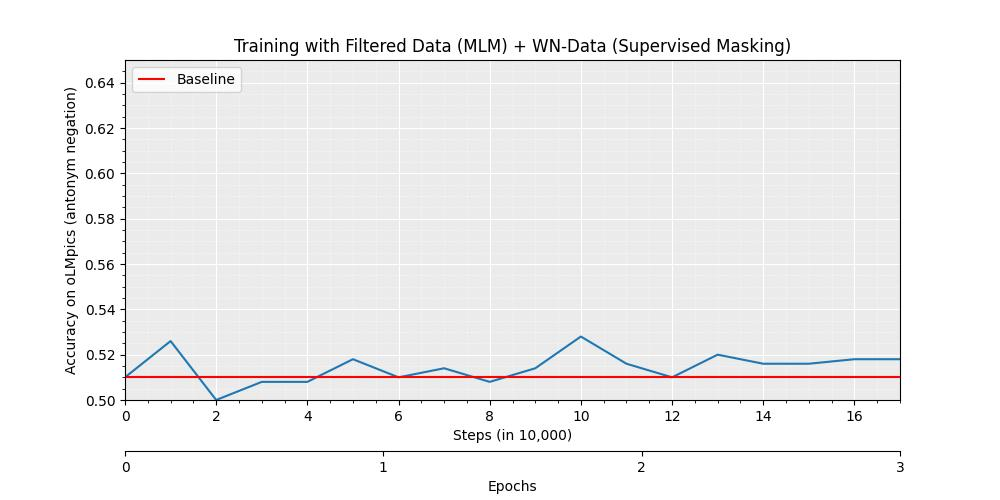
\includegraphics[width=\textwidth]{figures/Training_with_Filtered_Data__MLM____WN_Data__Supervised_Masking_.jpg}
    \caption{Experiment 2: Training BERT-Small on the filtered dataset using unsupervised MLM and the WordNet adversarial dataset using supervised masking.}
    \label{fig:graph_exp2}
\end{figure}



\subsection{Hyperparameters - Experiment 3}
\begin{table}[!h]
    \centering
    \begin{tabular}{r|l}
        Parameter & Value \\ \hline
        Model Identifier (transformers library) & \texttt{prajjwal1/bert-small} \\
        Optimizer & AdamW \\
        Learning Rate & 5e-5 \\
        Epochs & 3 \\
        Batch Size & 24 \\
        Blocksize & 128 \\
        Data Collator for Training & \texttt{DataCollatorForLanguageModeling} (transformer library) \\
        Test Ds. Proportion & 5 \\
        Steps (Evaluation) & 10000 \\
        seed & 23, 42, 7\\
        Layers Frozen & 0, 1, 2 \\
         \multirow{16}{*}{Frozen Layers} &     bert.encoder.layer.\{0,1,2,\}.attention.self.query.weight \\
                      &      bert.encoder.layer.\{0,1,2,\}.attention.self.query.bias \\
                      &      bert.encoder.layer.\{0,1,2,\}.attention.self.key.weight \\
                      &      bert.encoder.layer.\{0,1,2,\}.attention.self.key.bias \\
                      &      bert.encoder.layer.\{0,1,2,\}.attention.self.value.weight \\
                      &      bert.encoder.layer.\{0,1,2,\}.attention.self.value.bias \\
                      &      bert.encoder.layer.\{0,1,2,\}.attention.output.dense.weight \\
                      &      bert.encoder.layer.\{0,1,2,\}.attention.output.dense.bias \\
                      &      bert.encoder.layer.\{0,1,2,\}.attention.output.LayerNorm.weight \\
                      &      bert.encoder.layer.\{0,1,2,\}.attention.output.LayerNorm.bias \\
                      &      bert.encoder.layer.\{0,1,2,\}.intermediate.dense.weight \\
                      &      bert.encoder.layer.\{0,1,2,\}.intermediate.dense.bias \\
                      &      bert.encoder.layer.\{0,1,2,\}.output.dense.weight \\
                      &      bert.encoder.layer.\{0,1,2,\}.output.dense.bias \\
                      &      bert.encoder.layer.\{0,1,2,\}.output.LayerNorm.weight \\
                      &      bert.encoder.layer.\{0,1,2,\}.output.LayerNorm.bias \\
    \end{tabular}
    \caption{Hyperparameters used in Experiment 3. All values that are not reported, are default values from the transformer library.}
    \label{tab:hyp_exp3}
\end{table}

\newpage

\subsection{Evaluation Graph - Experiment 3}
\begin{figure}[!h]
    \centering
    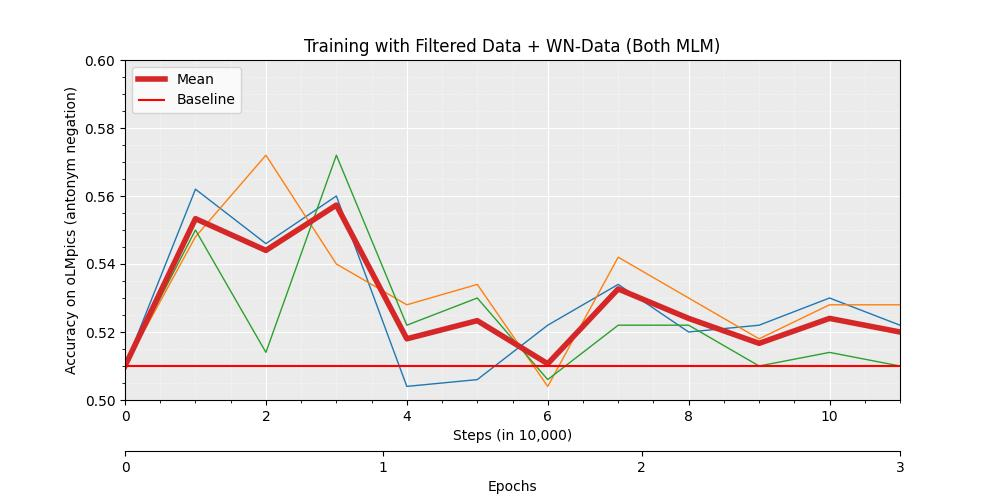
\includegraphics[width=\textwidth]{figures/FiltWNMixed.jpg}
    \caption[width=\textwidth]{Experiment 3: Training BERT-Small on the filtered dataset and the WordNet adversarial dataset using unsupervised MLM. The yellow, green, and blue lines represent the different training runs using different seeds.}
    \label{fig:graph_exp3}
\end{figure}
\newpage

\subsection{Hyperparameters - Experiment 3+}
\begin{table}[!h]
    \centering
    \begin{tabular}{r|l}
        Parameter & Value \\ \hline
        Model Identifier (transformers library) & \texttt{prajjwal1/bert-small} \\
        Optimizer & AdamW \\
        Learning Rate & 5e-5 \\
        Epochs & 3 \\
        Batch Size & 24 \\
        Blocksize & 128 \\
        Data Collator for Training & \texttt{DataCollatorForLanguageModeling} (transformer library) \\
        Test Ds. Proportion & 5 \\
        Steps (Evaluation) & 10000 \\
        seed & 42 \\
        Layers Frozen & 0, 1, 2 \\
         \multirow{16}{*}{Frozen Layers} &     bert.encoder.layer.\{0,1,2,\}.attention.self.query.weight \\
                      &      bert.encoder.layer.\{0,1,2,\}.attention.self.query.bias \\
                      &      bert.encoder.layer.\{0,1,2,\}.attention.self.key.weight \\
                      &      bert.encoder.layer.\{0,1,2,\}.attention.self.key.bias \\
                      &      bert.encoder.layer.\{0,1,2,\}.attention.self.value.weight \\
                      &      bert.encoder.layer.\{0,1,2,\}.attention.self.value.bias \\
                      &      bert.encoder.layer.\{0,1,2,\}.attention.output.dense.weight \\
                      &      bert.encoder.layer.\{0,1,2,\}.attention.output.dense.bias \\
                      &      bert.encoder.layer.\{0,1,2,\}.attention.output.LayerNorm.weight \\
                      &      bert.encoder.layer.\{0,1,2,\}.attention.output.LayerNorm.bias \\
                      &      bert.encoder.layer.\{0,1,2,\}.intermediate.dense.weight \\
                      &      bert.encoder.layer.\{0,1,2,\}.intermediate.dense.bias \\
                      &      bert.encoder.layer.\{0,1,2,\}.output.dense.weight \\
                      &      bert.encoder.layer.\{0,1,2,\}.output.dense.bias \\
                      &      bert.encoder.layer.\{0,1,2,\}.output.LayerNorm.weight \\
                      &      bert.encoder.layer.\{0,1,2,\}.output.LayerNorm.bias \\
        Amount (For WN Data Generation)  & 10 \\
    \end{tabular}
    \caption{Hyperparameters used in Experiment 3. All values that are not reported, are default values from the transformer library.}
    \label{tab:hyp_exp3+}
\end{table}

\subsection{Hyperparameters - GLUE-Fine-Tuning}
\begin{table}[!h]
    \centering
    \begin{tabular}{r|l}
        Parameter & Value \\ \hline
        Learning Rate & 2e-5 \\
        Batch Size & 16 \\
        Weight Decay & 0.1 \\
        Epochs & 10 \\
        Warmup Ratio & 0.06 \\
    \end{tabular}
    \caption{Hyperparameters used in fine-tuning selected GLUE tasks. All values that are not reported are default values from the transformer library.}
    \label{tab:glue-ft}
\end{table}

\end{document}
